%--------------------
% Packages
% -------------------
\documentclass[11pt,a4paper]{article}
\usepackage[utf8x]{inputenc}
\usepackage[T1]{fontenc}
%\usepackage{gentium}
\usepackage{mathptmx} % Use Times Font
\usepackage{esvect}
\usepackage{mathrsfs}
\usepackage{axodraw2}

%\usepackage[pdftex]{graphicx} % Required for including pictures
\usepackage[pdftex,linkcolor=black,pdfborder={0 0 0}]{hyperref} % Format links for pdf
\usepackage{calc} % To reset the counter in the document after title page
\usepackage{enumitem} % Includes lists

\frenchspacing % No double spacing between sentences
\linespread{1.2} % Set linespace
\usepackage[a4paper, lmargin=0.1666\paperwidth, rmargin=0.1666\paperwidth, tmargin=0.1111\paperheight, bmargin=0.1111\paperheight]{geometry} %margins
%\usepackage{parskip}

\usepackage[all]{nowidow} % Tries to remove widows
\usepackage[protrusion=true,expansion=true]{microtype} % Improves typography, load after fontpackage is selected

\usepackage{lipsum} % Used for inserting dummy 'Lorem ipsum' text into the template


%-----------------------
% Set pdf information and add title, fill in the fields
%-----------------------
\hypersetup{ 	
pdfsubject = {The Discovery of Dark Matter - NOTES},
pdftitle = {},
pdfauthor = {}
}

%-----------------------
% Begin document
%-----------------------
\begin{document} %All text i dokumentet hamnar mellan dessa taggar, allt ovanför är formatering av dokumentet

\section{On Particle Physics}
\subsection{Standard Model}
\subsection{Cross Sectional Area}
Propagator:
\begin{equation}
    \frac{1}{s} = \frac{1}{q_0^2 - |q|^2} = \frac{1}{{E^{TOT}_{CoM}}^2}
\end{equation}

\subsection{Luminosity}
Luminosity $\mathscr{L}$, is number of collisions per unit area per second (number of events that will be observed), quoted in $cm^{-2}s^{-1}$. A higher luminosity means greater likelihood particles will collide and result in a desired interaction

\subsubsection{Connection with Cross sectional area, $\sigma$}
Luminosity measures how many particles pass through a square centimetre per second. Cross section measures
the likelihood that a desired event will happen. These two are inversely related in that the luminosity times the
cross section gives the number of expected events per second.

rate of reaction, $R = \frac{dN}{dt} = \mathscr{L} x \sigma$

see: \url{https://cds.cern.ch/record/2800578/files/Cross%20Section%20and%20Luminosity%20Physics%20Cheat%20Sheet.pdf}

integrated luminosity, $L = \int \mathscr{L} dt$
total number of events, $N = \int (\mathscr{L} x \sigma) dt$, with error of $\sqrt{N}$, and accuracy of $\frac{1}{\sqrt{N}}$.

luminosity is proportional to the square of the number of particles in each beam, $n$, the revolution frequency, $f$, number of particles in each beam, $N_1$ and $N_2$, and inversely proportional to the beam cross section $A$.
\begin{equation}
    \mathscr{L} = \frac{n^2 f N_1 N_2}{A}
\end{equation}
\subsection{Feynman Rules}
To obtain the amplitude of an interaction, there are some rules used. For an EM interaction:
\begin{itemize}
    \item Vertex is proportional to the charge
    \item Conservation of E and $\vec{p}$ at each vertex
    \item The propagator: 
        \begin{equation}
            D(q_o, \vec{q}) = \frac{1}{q_0^2 - |\vec{q}|^2 - M + i\Gamma M}
        \end{equation}
        Where $q_0 = \frac{(E^1 _f - E^1 _i)}{c} = \frac{(E^2 _f - E^2 _i)}{c}$
        and $\vec{q} = \vec{p}^1_f - \vec{p}^1_i = \vec{p}^2_f - \vec{p}^2_i$
\end{itemize}
And so the amplitude of the interaction, $\mathscr{A}$ is proportional to:
\begin{equation}
    \frac{e_1 e_2}{q_0^2 - |\vec{q}|^2} = \frac{e_1 e_2}{\frac{(E^1 _f - E^1 _i)}{c} - \vec{p}^1_f - \vec{p}^1_i}
\end{equation}

And we can say that $\mathscr{A} \propto \frac{e^2}{s}$

\begin{figure}[h]
    \centering
    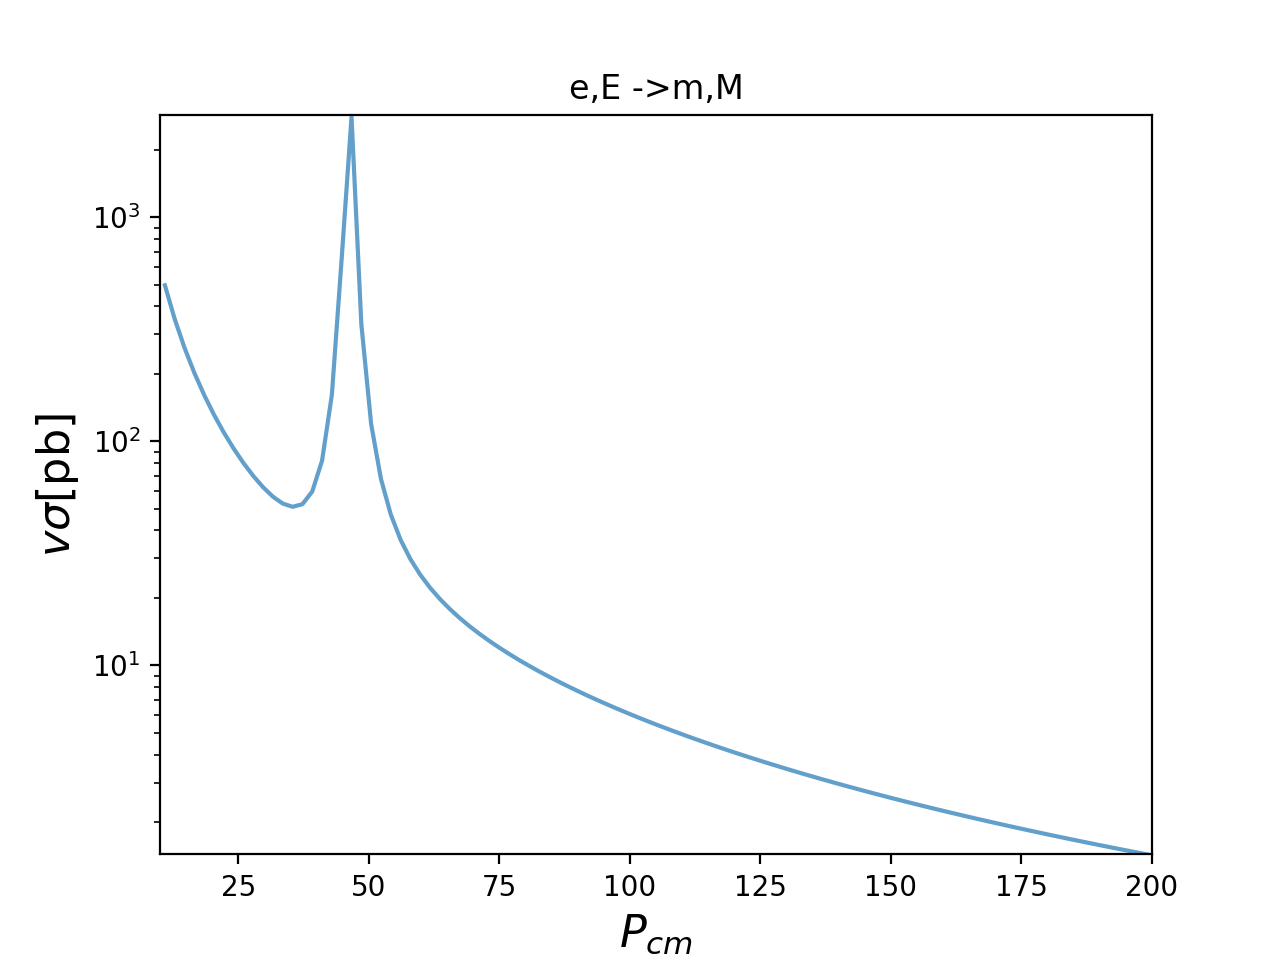
\includegraphics[width=0.5\linewidth]{Documents/Notes/Fig/eE-mM.png}
    \caption{Cross sectional area of interaction between $e^-$, $e^+$ annihilating to give $\mu^+$ $\mu^-$. The resonance peak is the energy of the $Z^0$ boson}
    \label{fig:enter-label}
\end{figure}

\subsection{Interactions}
\subsubsection{Electromagnetic}
Intermediate particle (virtual particle): EM wave, $\gamma$
Conservation Laws:
\begin{itemize}
    \item E, $\vec{p}$ at each vertex
    \item Charge, Q
    \item Lepton number ($L_{e^-} = +1$, $L_{e^+} = -1$)
    \item Flavour
\end{itemize}

\subsubsection{Strong}
Intermediate particle (virtual particle): Gluon, g
\begin{itemize}
    \item E, $\vec{p}$ at each vertex
    \item Flavour
\end{itemize}
Note: No electric charges in play, and leptons do not interact strongly.

\subsubsection{Weak (Neutral)}
Intermediate particle (virtual particle): Z boson, $Z^0$
Similar conservation laws to EM:
\begin{itemize}
    \item E, $\vec{p}$ at each vertex
    \item Charge, Q
    \item Lepton number
    \item Flavour
\end{itemize}

\subsubsection{Weak (Charged)}
Intermediate particle (virtual particle): W boson, $W^+$ or $W^-$
Conservation laws:
\begin{itemize}
    \item E, $\vec{p}$ at each vertex
    \item Charge, Q
    \item Lepton number
\end{itemize}

\subsection{Feynman Diagrams}
{
\unitlength=1.0 pt
\SetScale{1.0}
\SetWidth{0.7}      % line    size control
\scriptsize    %  letter  size control
{} \qquad\allowbreak
%  diagram # 1
\begin{picture}(96,38)(0,0)
    \ArrowLine(12.0,35.0)(36.0,23.0) 
    \Text(12.0,35.0)[r]{$e$}
    \ArrowLine(36.0,23.0)(12.0,11.0) 
    \Text(12.0,11.0)[r]{$E$}
    \DashLine(36.0,23.0)(60.0,23.0){3.0} 
    \Text(49.0,24.0)[b]{$A$}
    \ArrowLine(60.0,23.0)(84.0,35.0) 
    \Text(84.0,35.0)[l]{$m$}
    \ArrowLine(84.0,11.0)(60.0,23.0) 
    \Text(84.0,11.0)[l]{$M$}
\end{picture} \ 
{} \qquad\allowbreak
%  diagram # 2
\begin{picture}(96,38)(0,0)
    \ArrowLine(12.0,35.0)(36.0,23.0) 
    \Text(12.0,35.0)[r]{$e$}
    \ArrowLine(36.0,23.0)(12.0,11.0) 
    \Text(12.0,11.0)[r]{$E$}
    \DashLine(36.0,23.0)(60.0,23.0){3.0} 
    \Text(49.0,24.0)[b]{$Z$}
    \ArrowLine(60.0,23.0)(84.0,35.0) 
    \Text(84.0,35.0)[l]{$m$}
    \ArrowLine(84.0,11.0)(60.0,23.0) 
    \Text(84.0,11.0)[l]{$M$}
\end{picture} \ 
}

\section{Dark Matter}
Initially, universe hot with initial temp unknown (big bang, dont know when and how hot. we know for sure it was above 10MeV, otherwise big bang will not happen). This
should be sufficiently hot to generate protons and neutrons.
strong confidence that there was inflation (big bang was an expansion from a singularity which slowed down over time)
all particles in plasma in thermal equilibrium. energy of plasma -> high enough to produce particles ($E = mc^2$)
assume DM is particles. and DM interact with particles. 

At high enough temps (higher than their mass) they behave relativistic and behave similarly (same number of dof (1-3 factor difference))
universe cooling down, temp drops exponentially ~14 billion years to current day.
at some point the temperature became lower than DM mass, meaning it can annihilate with SM particles (however, there is no reverse process. (freeze out process))
dark matter -> sm particles, no way around. depending on c.s, relic density can be derived. higher rate, the less DM there is.
dm density drops due to annihilation. reaction rate becomes smaller than the rate of expansion of the universe. then DM canot annihilate anymore due to low density. then dm density ~ constant (freeze out)
if DM annihilates too strongly, no relic DM left. If DM reacts too weakly, there will be too little DM, and the universe will be filled with too much DM -> universe closes up
controlled by Boltzmann equation (classical) to know the rate of reaction. 
freeze in - if DM interacts with SM particles weakly, at high temps SM particles and DM will not be in thermal equilibrium (since they react weakly). rarely that SM particles react with DM. 

\section{Detection of Dark Matter}
\subsection{Direct}
Underground Dirac detection
\subsection{Indirect}
Collider search, where:
\begin{itemize}
    \item $E = mc^2$, can derive mass of DM from energy of collider
    \item A visible particle is recoiled by an invisible particle
    \item Missing momenta can deduce mass of Dark matter
\end{itemize}
\section{}


\section{CalcHEP Notes}


\end{document}

